% 原书第 3—6 页；章首导言及第 1.1—1.2 节。
\chapter{数据科学中的研究问题}
\label{ch:research-questions-data-science}
\chapterauthors{Sherri Rose 与 Mark J. van der Laan}
\chapteraffiliations{%
S. Rose（通讯作者）：美国哈佛医学院卫生保健政策系，180 Longwood Ave, Boston, MA 02115, USA；电子邮箱：\href{mailto:rose@hcp.med.harvard.edu}{rose@hcp.med.harvard.edu}。\\
M. J. van der Laan：美国加利福尼亚大学伯克利分校生物统计学部及统计学系，101 Haviland Hall, \#7358, Berkeley, CA 94720, USA；电子邮箱：\href{mailto:laan@berkeley.edu}{laan@berkeley.edu}。\\
本章 DOI：\url{https://doi.org/10.1007/978-3-319-65304-4_1}。}

随着我们获取新型数据的能力不断增强，医学、技术和商业领域所面临的研究问题也日益复杂。观察性研究（observational study）和实验性研究中的许多数据，都是经过长期收集而得到的，其间还会在多个时点采集多项测量值。这些数据有些是流式数据，例如 Twitter 上的帖子，也有图像、DNA 序列和电子健康记录。我们必须发展和调整统计学习（statistical learning）方法，以应对这些新的挑战。

2010 年，Google Flu Trends（谷歌流感趋势）被誉为集体智慧的杰出范例。研究人员声称，他们利用数百万条用户搜索词预测二十多个国家的流感情况，准确率达到 97\%，而且比美国疾病控制与预防中心提前两周识别出流感病例的激增。然而，人们很快发现，这些技术经常高估流感流行程度，将多种疾病混为一谈，并存在严重的数据过拟合问题。目前，这一项目已不再公开运行。

奖金高达 100 万美元的 Netflix Prize（奈飞大奖赛）同样在媒体和数据科学界引起了轰动。比赛向能够改进其电影推荐算法的团队提供高额奖金。获胜团队开发的算法使 Netflix 推荐系统的表现提高了 10\%。然而，由于部署该算法所涉及的工程问题过于复杂，Netflix 从未真正采用获胜团队的算法。尽管存在这一失败，该奖项仍不断被赞誉为展现大数据与数据科学协作团队潜力的典型范例。

数据科学正在走向这样的分析系统：它融合统计学、机器学习（machine learning）和计算机科学领域的进展，能够对大型数据集中的感兴趣量进行快速而稳健的估计。上述两个近期案例表明，这类大数据系统既需要以统计理论为基础的方法论，也需要快速、灵活且切实可行的计算实现。本书围绕靶向学习（targeted learning）展开，与这些目标相一致。我们将介绍适用于大数据的经验方法，用来估计一系列复杂参数，同时保证计算上的可行性。

\section{从（大）数据中学习}
\label{sec:ch01-learning-from-data}

靶向学习关注基于机器学习的有效代入估计量（substitution estimator），所估计的参数被定义为数据概率分布的某种特征；同时，它还通过自助法（bootstrap）或影响曲线（influence curve）提供统计推断。靶向学习是一个广泛的框架，其中既包括用于效应估计问题的靶向极大似然估计量（targeted maximum likelihood estimator，TMLE），也包括用于预测的超级学习（super learning），后者是一种集成机器学习技术。TMLE 以无限维参数的基于损失的估计文献为基础，将估计靶向于效应参数等较低维参数。这些估计量经过专门构造，能够消除目标效应特征所剩余的偏差。超级学习完全融入 TMLE 算法相关组成部分的估计之中。TMLE 具有许多理想的统计性质，包括双重稳健性（double robustness），而且是定义良好的代入估计量。靶向学习以其独特方式解决了一项巨大挑战：将数据自适应估计（data-adaptive estimation）与正式的统计推断结合起来。

\begin{sourcebox}
科学界一直在共同努力，解决可能影响研究可靠性的诸多问题，包括实验性和非实验性研究的设计，以及用于评价这些研究的统计分析。靶向学习在这一领域发挥着关键作用：它强调预先指定的分析方案和算法，在更为灵活的非参数或半参数统计模型（nonparametric or semiparametric statistical model）中作出现实的假设。其目标是利用我们关于数据及其背后数据生成机制（data-generating mechanism）的知识，精确描述观测单位和模型，并将研究问题准确转化为统计估计问题。随后，靶向统计学习机器以我们的数据和知识作为系统输入，采用事先严格指定的评价基准和具有理论基础的估计量，生成可解释且与政策相关的结果。
\end{sourcebox}

\begin{center}
 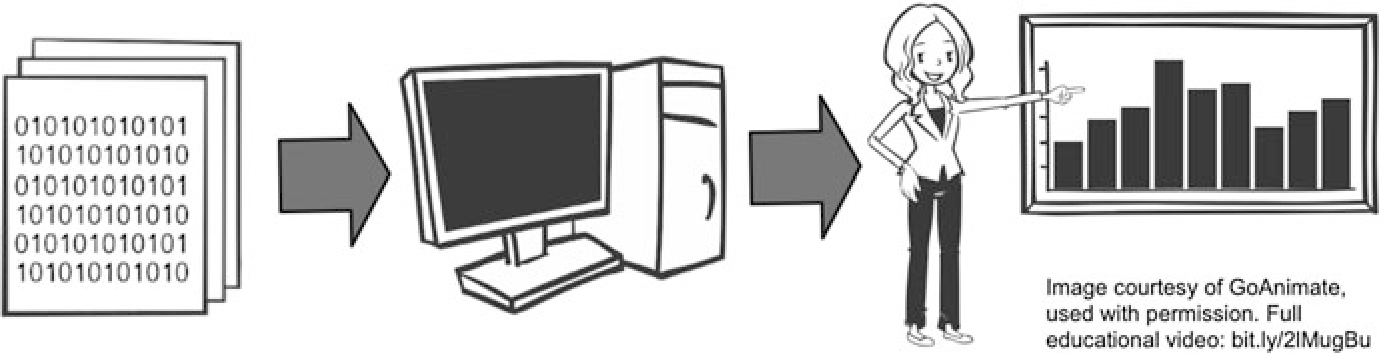
\includegraphics[width=.91\textwidth]{figures/ch01_unnumbered_workflow.png}\\[-.2em]
 {\footnotesize 图片由 GoAnimate 提供，经授权使用。完整教学视频：\url{https://bit.ly/2lMugBu}。}
\end{center}

\begin{sourcebox}
\kaishu 这一切都以计算效率和实际应用为重。其理念是：从理论上最优的方法出发，确保将其转化为快速、便于用户使用的工具。
\end{sourcebox}

过去十年间，靶向学习已经发展为构造效应估计量和预测函数的可靠框架。随着靶向学习不断发展，它不仅为许多数据结构中的现有问题提供了新的解决方法，也在不同应用领域带来了新的发现。相关研究涉及随机对照试验（randomized controlled trial）、由边际结构模型（marginal structural model）定义的参数、病例对照研究、协同 TMLE（collaborative TMLE）、缺失和删失数据、纵向数据（longitudinal data）、效应修饰、比较效果研究、衰老、癌症、职业暴露、医保计划支付风险调整以及 HIV 等。在许多情况下，这些研究将靶向学习技术与标准方法进行了比较，表明它在模拟研究和现实应用中具有更好的表现。

\section{传统估计方法的失效}
\label{sec:ch01-traditional-fail}

经典横断面研究已有许多可用的方法，例如传统参数回归和若干现成的统计机器学习技术；然而，对于数据科学各领域中的复杂纵向研究，相关方法却十分匮乏。这些方法在横断面研究中就会失效，其假设也会不成立；将它们用于涉及时变处理、网络或流式数据等复杂数据类型时，问题会进一步加剧。本书旨在弥补这一缺口，介绍为处理此类难题而专门设计的靶向学习方法。第一部《靶向学习》讨论了前述横断面研究方法，也介绍了最早用于纵向研究的 TMLE 估计量，展示了靶向学习方法在多种数据结构中的优势。本书进一步介绍新的进展，因此采用了《复杂纵向研究的因果推断》这一副标题。

人们还普遍认为，在非参数或半参数模型中，采用数据自适应的估计，也就是基于机器学习的估计时，无法进行统计推断。让我们更具体地说明这一点。假设在一项观察性研究中，我们已经使用机器学习，将临床结局的条件均值拟合为处理与患者特征的函数。为此，我们可以采用集成学习器（ensemble learner），例如超级学习器：它结合算法库中的多个算法，并依赖交叉验证（cross-validation）。然后，通过以下两步，将这一拟合结果映射为特定处理下均值（treatment-specific mean）的估计：（1）计算指定处理条件下的预测结局；（2）在样本的全部 $n$ 名研究对象中，对这些预测值取平均。

以往的常规做法并不是使用机器学习，而是根据参数回归模型，用极大似然估计量来估计回归函数。在这种情形下，所得特定处理下均值，是未知回归系数的极大似然估计量的一个简单函数。因此，如果回归模型设定正确，特定处理下均值的这一极大似然估计量就是渐近线性的（asymptotically linear）。（这意味着，该极大似然估计量减去真实的特定处理下均值，等于其影响曲线的经验均值再加上一个可忽略的余项。）由此，它近似服从正态分布，其均值为真实的特定处理下均值，方差为影响曲线的方差除以样本量。置信区间的构造与基于样本均值的置信区间类似。然而，在实际中，我们知道这一参数模型存在设定错误，因此，该极大似然估计量虽服从正态分布，却带有偏差，95\% 置信区间的渐近覆盖率将等于零。

如果像前面最初提出的那样使用机器学习算法，那么，特定处理下均值的估计量一般不服从正态分布，且偏差大于 $1/\sqrt{n}$。因此，用 $\sqrt{n}$ 标准化之后，估计量与其真值之差将趋于无穷！由于估计量的抽样分布通常无法用某个给定分布（例如正态分布）很好地近似，我们也就无法根据这样的极限分布进行统计推断。

值得注意的是，只要对基于机器学习的拟合结果作一个小幅的靶向修正，就可能使所得特定处理下均值的估计量具有渐近线性，且其影响曲线等于有效影响曲线（efficient influence curve）。这里的初始估计量（initial estimator）估计的是数据分布，或其相关部分，例如本例中的回归函数；将它代入目标参数（target parameter）时，所得估计量通常偏差过大，而且不服从正态分布。这一小幅修正能够把初始估计量映射为更新后的估计量，使相应的代入估计量近似无偏，并具有方差最小的正态极限分布。
